\documentclass[11pt,a4paper,openright]{report}
\usepackage{float}
\usepackage{amsmath}
\usepackage{booktabs}
\usepackage{graphicx}
\usepackage{listings}
\usepackage{graphicx}
\usepackage{pst-rel-points}
\usepackage{pstricks}
\usepackage{pst-node}
\usepackage{pst-text}
\usepackage{auto-pst-pdf}
\usepackage{etex}
\usepackage{verbatim}
\usepackage{pgfplots} 
\usepackage{courier}
\lstset{basicstyle=\footnotesize\ttfamily}

\pgfplotsset{width=10cm,compat=1.5}
\restylefloat{table}
%\usepackage{ps2pdf}

%%\lstset{language=C}
\title{\textbf{Liveness-based Reaching Definition Analysis using PRISM}}
\vspace{2.5cm}
\author{\emph{by}\\ \\ \bf{Rashmi Rekha Mech}\\\bf{Roll No : 133050089} \\
\\ \emph{Under the Guidance of}\\ \\\textbf{Prof. Uday Khedker}\\}
\date{}


\begin{document}
\maketitle
\begin{abstract}
 This document provides an updates on implemented liveness-based inter-procedural reaching definition analysis. It also provides some data (SPEC Benchmark) to compare 
 with and without liveness-based reaching definition analysis. It also presents some issues in doing pointer analysis. 
\end{abstract}




\maketitle
%\begin{comment}
%%%%%%%%%%%%%%%%%%%%%%%%%%%%%%%%%%%%%%%%%%%%%%%%%%%%%%%%%%%%%%%%%%%%%%%%%%%%%
\section*{Description}
In liveness-based reaching definition analysis, a definition $d_x: x=e$ reaches a program point $u$ if it appears (without a redefinition of $x$) on some path from program 
entry to $u$ and $x$ is live at $u$. Context sensitive analysis results in more precise information, therefore for inter-procedural analysis we are using context sensitive 
inter-procedural analysis implemented by Vinit. 

Data flow equations for Liveness-based reaching definition analysis :
\begin{equation}
\begin{split}
\mbox{\textit{LIn}}_n &= f_n(\mbox{\textit{Out}}_n) \\
\mbox{\textit{LOut}}_n &= \left\{ \begin{array}{ll}
	  BI & \mbox{n is End}\\
	  \bigcup\limits_{s \in succ(n)} In_s & \mbox{otherwise}
	  \end{array} \right.\\ 
\mbox{where,}\\
f_n(X) &= \left\{ \begin{array}{ll}
	  (X-\{y\})\cup(\mbox{\textit{Opd(e)}}\cap \mbox{\textit{Var}}) & \mbox{n is y = e, e $\in$ Expr, y $\in$ X}\\
	  X-{y} & \mbox{n is input(y)}\\
	  X \cup {y} & \mbox{n is use(y)} \\
	  X & \mbox{otherwise}
	  \end{array} \right.\\ 
\\
\mbox{\textit{RIn}}_n &= \left\{ \begin{array}{ll}
	  \mbox{\textit{RBI}} & \mbox{n is Start block}\\
	  \bigcup\limits_{p \in pred(n)}Out_p\mid_{LIn_n} & \mbox{otherwise}
	  \end{array} \right.\\ 
	  \\
\mbox{\textit{ROut}}_n &= \mbox{\textit{Gen}}_n \cup (\mbox{\textit{In}}_n - \mbox{\textit{Kill}}_n) \mid_{LOut_n} \\
\\
\mbox{\textit{RBI}} &= \{d_x : x = \mbox{\textit{undef}} \mid x \in \mbox{\textit{Var}}\} \\	  
\end{split} 
\end{equation}



\section*{SPEC Benchmark Evaluation}
In order to compare the performance between two analysis i.e. inter-procedural reaching definition analysis with and without liveness, we tested both for SPEC Benchmarks.
For each query, we measured the average size of the set of data flow values computed at each program point. In general, average size of the set at each
program point in liveness-based analysis is much smaller than that of the normal reaching definition analysis.

Performance measurement of reaching definition without liveness is shown in table~\ref{tab:performance_without_l}.
\begin{table}[H]
  \begin{center}
      %\label{tab:Available_exp}
    \begin{tabular}{|c|p{1.5cm}|p{2cm}|p{2cm}|p{2cm}|}
    \hline
%        & \multicolumn{2}{c}{$a+b$} & \multicolumn{2}{c}{$a*b$} & \multicolumn{2}{c}{$a*c$} \\
%     \hline
      Name & No. of Basic Blocks & Avg. values at Entry & Avg. values at Exit & Total values \\
      \hline
%    	\midrule
   	  bzip2 & 8004 & 113.89 & 114.18 & 114.04 \\ \hline
   	  mcf & 1066 & 94.90 & 95.01 & 94.96 \\ \hline
   	  hmmer & 24996 & 57.53 & 57.70  & 57.61 \\ \hline
   	  sjeng & 10892 & 39.219 & 39.245 & 39.232 \\ \hline
   	  lbm & 603 & 10.53 & 10.71 & 10.62\\ \hline
   	  
	\hline
%       \bottomrule 
    \end{tabular}
    \caption{Benchmark results for normal reaching definition analysis.}
      \label{tab:performance_without_l}
  \end{center}
\end{table}

The performance measurement of reaching definition with liveness is shown in table~\ref{tab:performance_with_l}.
\begin{table}[H]
  \begin{center}
      %\label{tab:Available_exp}
    \begin{tabular}{|c|p{1.5cm}|p{2cm}|p{2cm}|p{2cm}|}
    \hline
%        & \multicolumn{2}{c}{$a+b$} & \multicolumn{2}{c}{$a*b$} & \multicolumn{2}{c}{$a*c$} \\
%     \hline
      Name & No. of Basic Blocks & Avg. values at Entry & Avg. values at Exit & Total values\\
      \hline
%    	\midrule
   	  bzip2 & 8004 & 10.45 & 10.23 & 10.34 \\ \hline
   	  mcf & 1066 &  22.07 & 21.77 & 21.92 \\ \hline
   	  hmmer & 24996 & 1.38 & 1.34  & 1.36 \\ \hline
   	  sjeng & 10892 & 11.96 & 11.69 & 11.82 \\ \hline
   	  lbm & 603 & 1.50 & 1.46 & 1.48\\ \hline
   	  
	\hline
%       \bottomrule 
    \end{tabular}
    \caption{Benchmark results for liveness-based reaching definition analysis.}
      \label{tab:performance_with_l}
  \end{center}
\end{table}

Figure~\ref{fig:bench_mark} shows a comparision between two analysis.
\begin{figure}[H]
\centering
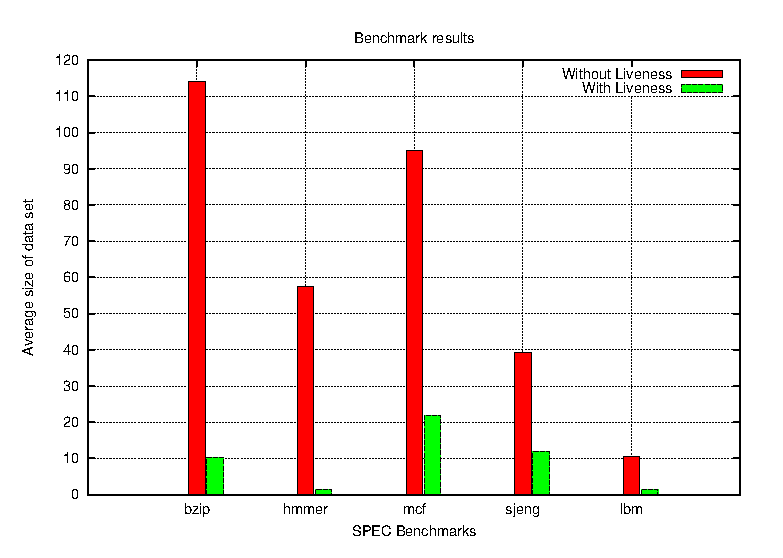
\includegraphics[width=0.8\textwidth]{graph_new.eps}
\caption{Percentage reduction in size of data set for Reaching definition analysis with and without liveness}
\label{fig:bench_mark}
\end{figure}


\section*{Difficulties}

We need pointer information for expressions containing pointer variables but due to some changes in solver, the old alias query produces an empty result.
To solve this problem, we are computing a set of pointer information at each program point by using Vinit's pointer analysis query. Also, we are only able to run 
five SPEC Benchmarks as shown in the tables ~\ref{tab:performance_without_l} and ~\ref{tab:performance_with_l}. 
We are not able to run the following Benchmarks :
\begin{itemize}
 \item 464.h264ref : It is taking a long time to execute. Large number of pointers availble in this Benchmark may be the reason for taking long time to execute.
 \item 403.gcc : It gives error in opening ``sbitmap.st'' file. This file is not generated during IR generation.
 \item 462.libquantum : This is also giving the same error ``error in opening shor.st file ''.
 \item 433.milc : This is also giving the same error ``error in opening control.st file ''.

\end{itemize}





%%%%%%%%%%%%%%%%%%%%%%%%%%%%%%%%%%%%%%%%%%%%%%%%%%%%%%%%%%%%%%%%%%%%%%%%%%%%%

\end{document}
